\lecture{28}{Bose-Einstein Condensation}{Qiang Zhu}{scribe-name1,2,3}

\section{The statistical behavior for Bosons}
As said in the introduction of Fermions and Bosons, Quantum Statistics starts to play the role in the dense system and low temperatures.
For an electron at room temperature, the quantum volume is
\begin{equation}
\epsilon_0 = \frac{h^2}{8mL^2}(1^2+1^2+1^2) = \frac{3h^2}{8mL^2}
\end{equation}

\begin{equation}
N_0 = \frac{1}{e^{(\epsilon_0-\mu)/kT}-1}
\end{equation}

When T is very small, $N_0$ will be quite large. In this case, the denominator must be small,

\begin{equation}
N_0 = \frac{1}{1+(\epsilon_0-\mu)/kT-1} = \frac{kT}{\epsilon_0-\mu}  ~~~~(\textrm{when~} N_0 \gg 1)
\end{equation}

The chemical potential $\mu$ must be equal to $\epsilon_0$ at T=0, and just a bit less than $\epsilon_0$ at small T. To calculate the total energy of all electrons, we need to sum over the energies of the electrons in all occupied states. Now the question is \textbf{at which temperature we can observe that $N_0$ remains very large?}


\section{Computing the total number of Bosons}
\begin{equation}
N = \sum_s \frac{1}{e^{(\epsilon_s-\mu)/kT}-1}
\end{equation}

In practice, we can turn it to integral,
\begin{equation}
\label{eq0}
N = \int_0^\infty g(\epsilon)\frac{1}{e^{(\epsilon_s-\mu)/kT}-1}d\epsilon
\end{equation}

Where the $g(\epsilon)$ is the density of states. which has a similar function form following the electron gas model. 
\begin{equation}
g(\epsilon) = \frac{2}{\sqrt{\pi}}\bigg(\frac{2\pi m}{h^2}\bigg)^{3/2}V\sqrt{\epsilon}
\end{equation}

\begin{figure}[h]
\centering
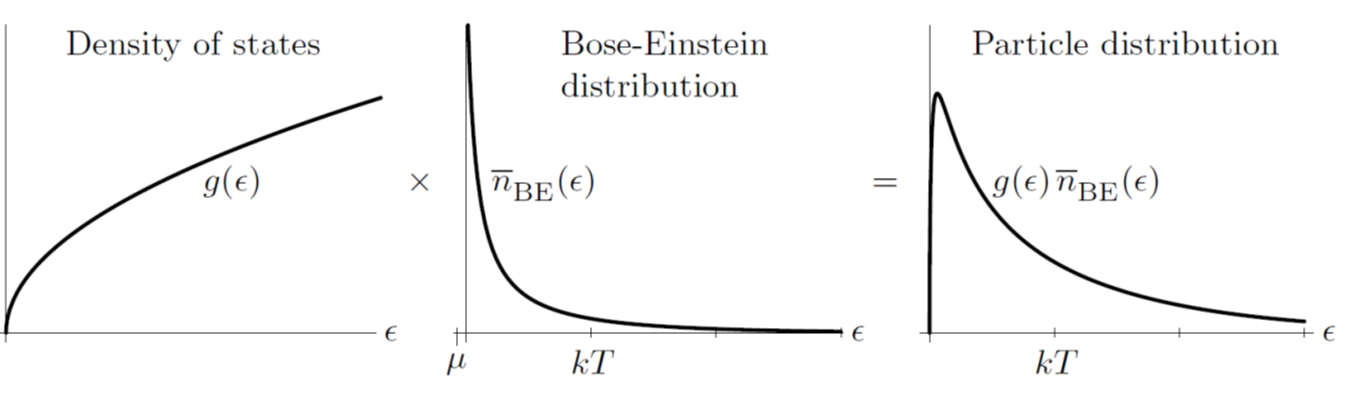
\includegraphics[width=0.9\linewidth]{imgs/BEC1.png}
\caption{The distribution of bosons as a function of energy is the product of
two functions, the density of states and the Bose-Einstein distribution. Copyright 2000, Addison-Wesley. }
\end{figure}

The trouble is that we cannot evaluate the eq.(\ref{eq0}) analytically. In order to work it out, we must guess some value for the $\mu$ term. A good starting point is let $\mu$=0. Changing the variable to $x = \epsilon/kT$
\begin{equation}
\begin{split}
    N = & \frac{2}{\sqrt{\pi}}\bigg(\frac{2\pi m}{h^2}\bigg)^{3/2}V \int_0^{\infty} \frac{\sqrt{\epsilon} d\epsilon}{e^{\epsilon/kT}-1}\\
      = & \frac{2}{\sqrt{\pi}}\bigg(\frac{2\pi mkT}{h^2}\bigg)^{3/2}V \int_{0}^{\infty} \frac{\sqrt{x} dx}{e^x-1}\\
\end{split}
\end{equation}

The integral over $x$ gives 2.315, which leaves us with
\begin{equation}
N = 2.612\bigg(\frac{2\pi mkT}{h^2}\bigg)^{3/2}V
\end{equation}

This result is wrong! It means that the number of particles purely depends on $T$. In fact, there can be only one $T$ corresponds to this value.
\begin{equation}
    N = 2.612\bigg(\frac{2\pi m kT_c}{h^2}\bigg)^{3/2}V
\end{equation}

When $T<T_c$, this will be no longer valid during the transformation from summation to integral. This is because the terms from $\epsilon =0$ is missing. Therefore, it should be better expressed as
\begin{equation}
    N_\textrm{exited} = 2.612\bigg(\frac{2\pi mkT}{h^2}\bigg)^{3/2}V
\end{equation}

While the gap between $N$ and $N_\textrm{exited}$ is the number of atoms in the ground state.
\begin{equation}
    N_0 = N-N_\textrm{exited} = \bigg[1-\bigg(\frac{T}{T_c}\bigg)^{3/2}\bigg]N
\end{equation}

\begin{figure}[ht]
\centering
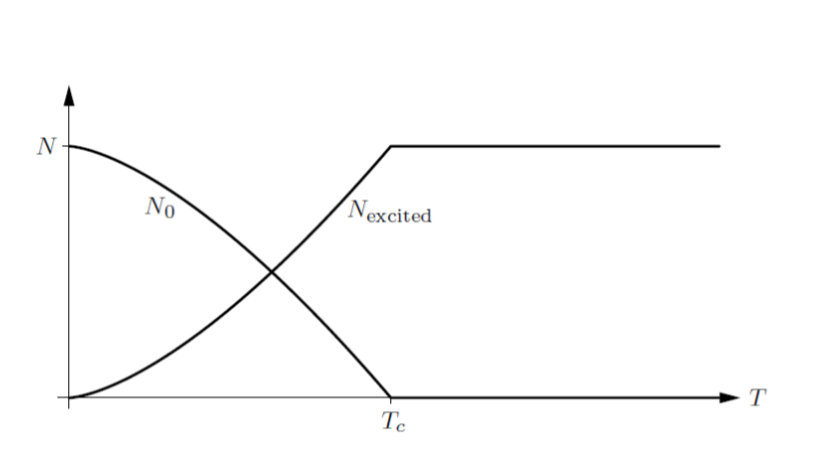
\includegraphics[width=0.8\linewidth]{imgs/BEC2.png}
\caption{Number of atoms in the ground state ($N_0$) and in excited states,
for an ideal Bose gas in a three-dimensional box. Below $T_c$ the number of atoms in excited states is proportional to $T^{3/2}$. Copyright 2000, Addison-Wesley}
\end{figure}

The abrupt accumulation of atoms in the ground state below $T_c$ is called \textbf{Bose-Einstein condensation}.

\section{Real World Examples}
In 1995 BEC of a gas of weakly interacting atoms was first achieved using Rb-87. Later, BEC was achieved with dilute gases of atomic Li, Na, H, .etc.

The superfluid phase of $^4$He is also considered to be the example of BEC.

\section{Why does it happen}



